\section{The MCG, FPG, and PSG}
    \label{s:building graphs}
We now discuss how the graph-based syntax defined in Secs.~\ref{s:syntax definition} and \ref{s:graph representation}  is used to represent an MDAO problem in its entirety. This discussion is based on the MCG and the FPG.

\subsection{Maximal Connectivity Graph}
    \label{ss:MCG}
For a specified MDAO problem, the maximal connectivity graph represents every analysis tool, objective, constraint, and input being considered, as well as every possible interconnection among them.
The definition of the MCG is given via construction.
    To construct the maximal connectivity graph, we presume that a set of analysis tools, inputs, objectives, and constraints are provided. 
    Each of the $m$ analysis codes correspond to an index $i\in I_A$, $I_A=\{1,2,\ldots,m\}$, and are represented by an analysis block graph $G_{A_i}=(V_{A_i},E_{A_i})$.
    Each of the $n$ expression blocks correspond to an index $i\in I_E$, $I_E=\{1,2,\ldots,n\}$, and is represented by expression block graph $G_{E_i}=(V_{E_i},E_{E_i})$.
    Finally, the inputs are represented as a set of variable nodes $V_\txt{in}$.
    We presume that $V_\txt{in}$, each $G_{A_i}$, and each $G_{E_i}$ are given, and that any potential connection between variables is specified in the form of connection edges in the set $E_{M,\txt{con}}$. One method for defining these connections is to use a consistant variable naming convention.

    We may then construct the maximal connectivity graph $M=(V_M,E_M)$ as
    \begin{IEEEeqnarray*}{rCl}
    V_M & = & V_\txt{in} \cup \left( \bigcup_{i \in I_A} V_{A_i} \right) \cup \left( \bigcup_{i \in I_E} V_{E_i} \right), \\
    E_M & = & E_{M,\txt{con}} \cup \left( \bigcup_{i \in I_A} E_{A_i} \right)  \cup \left( \bigcup_{i \in I_E} E_{E_i} \right).
    \end{IEEEeqnarray*}
    The MCG $M$ is uniquely determined by the given set of analysis blocks, inputs, and expression blocks. 
    In the cases where the set of inputs is not known a priori, the process of obtaining the FPG will reveal the required inputs, as discussed subsequently.

The nodes and edges in $M$ can be partioned in sets according to their type:
\begin{equation}
V_M = V_{M,\txt{var}} \cup V_{M,\txt{fun}}, \ V_{M,\txt{var}} \cap V_{M,\txt{fun}} = \emptyset,
\end{equation}
where $V_{M,\txt{var}}$ and $V_{M,\txt{mod}}$ are the sets of variable nodes and function nodes, respectively;
\begin{equation}
E_M = E_{M,\txt{con}} \cup E_{M,\txt{fun}}, \ E_{M,\txt{con}} \cap E_{M,\txt{fun}} = \emptyset,
\end{equation}
where $ E_{M,\txt{con}}$ and $E_{M,\txt{fun}}$ are the sets of connection edges and function edges, respectively. These sets will be referenced in the process for obtaining an FPG.

\subsection{Fundamental Problem Graph (FPG)}
    \label{ss:FPG}
    We now define the fundamental problem graph $F=(V_F,E_F)$ as a directed graph meeting the following conditions:
    \begin{enumerate}
    \item[(1)] $F \subset M$ and $G_{E_i} \subset F  \ \forall i \in I_E$
%    \item[(1)] $F \subset M$ and $V_\txt{out} \subset V_F$
    \item[(2)] $\displaystyle{\forall i \in I_A, \txt{ if } F \cap G_{A_i} \neq \emptyset \txt{ then } G_{A_i} \subset F}$
%    \item[(2)] $\displaystyle{\forall i \in I, \txt{ if } F \cap A_i \neq \emptyset \txt{ then } A_i \subset F}$
    \item[(3)] $\displaystyle{\forall v \in V_F \txt{ with }v \in V_{M,\txt{var}}}$ \txt{ and } \\
			 $\displaystyle{ \txt{deg}_l^-(v) \leq \txt{deg}^-(v) \leq \txt{deg}_u^-(v)}$
    \item[(4)] $\displaystyle{\forall v \in V_F \txt{ there exists a reverse path } P \subset R_F }$ \\
			$\displaystyle{\txt{ from } x \txt{ to } v \txt{ with } x\in V_{E_i}}$
%    \item[(4)] $\displaystyle{\forall v \in V_F \txt{ there exists a reverse path } P \subset R_F \txt{ from } x \txt{ to } v \txt{ with } x\in V_\txt{out}}$
    \end{enumerate}
    %The set $I_F$ is an index set containing the indices of the analysis blocks in $F$ and it may only include the analysis blocks $A_i$ that meet requirements (2) and (6). 
    %Requirement (2) stipulates that each analysis blocks in $F$ must have at least one local output that is being used. 
    %Requirement (3) stipulates that only the inputs that are being used should be included. 
    %Requirements (4) and (5) provide the construction of the sets of nodes and edges, respectively. 
    Condition (1) asserts that only the nodes and edges provided by the maximal connectivity graph can be used in the fundamental problem graph and that every expression block must be included. 
    Condition (2) requires that analysis blocks must be included or excluded in their entirety. 
    Condition (3) stipulates that the number of edges directed into each variable node must be within the lower and upper in-degree limits; 
    if $\txt{deg}^-(v) < \txt{deg}_l^-(v)$ the node is the location of a \emph{hole}, and if $\txt{deg}^-(v) > \txt{deg}_u^-(v)$ the node is the location of a \emph{collision}.
    Lastly, condition (4) ensures that only the nodes that are used in the MDAO problem formulation are included in the FPG by requiring that for every node a reverse path exists from at least one expression block to that node. 
    The reverse graph $R_F$ is obtained from $F$ by simply switching the orientation of every edge in $E_F$.

    %The set $C_F$ is a set containing connection edges representing connections. Since $C_M$ is the set of all potential connections, we must have $C_F \subset C_M$. 
    %While no other conditions are explicitly stated for $C_F$, requirement (6) is actually a requirement on both $I_F$ and $C_F$.

\subsection{Algorithm for Obtaining the Fundamental Problem Graph from the MCG}
    \label{ss:obtaining FPG}
    In general, there may be zero, one, or many graphs that satisfy the FPG conditions in Sec.~\ref{ss:FPG}.
    Here, we describe an algorithm for obtaining an FPG from a given MCG by starting with the MCG and disconnecting connection edges until the FPG conditions are met. 
    With this approach, the problem is reduced to deciding which connection edges to remove. 

\begin{description}
    \item[\bf{Step 1: Holes}] 
    The first step is to detect holes and disconnect the first set of connection edges 
    downstream of them, as indicated in Fig.~\ref{f:hole}. 

    To begin the process, an initial graph is created as a copy of the MCG
    \begin{equation}
    F_0 = M,
    \end{equation}
    where $F_0 = (V_{F_0},E_{F_0})$, and $C_{F_0,\txt{con}}$ is the set of connection edges. 
    The set of variable nodes that are holes is identified as
    \begin{equation}
    H = \{v \in V_{F_0} \st v \in V_{M,\txt{var}} \txt{ and } \txt{deg}^-(v) < \txt{deg}_l^-(v) \},
    \end{equation}
    which is the set of variable nodes with fewer incoming edges than are allowed by 
    the lower indegree limit. An updated set of edges is then created by removing the 
    connection edges preceding or succeeding the analysis block:
    \begin{IEEEeqnarray*}{rCl}
            E_{F_1} = E_{F_0} \setminus &\{& (x,y) \in E_{F_0,\txt{con}} \st x \in V_{A_i} \\
    & &  \txt{ or } y \in V_{A_i}, \txt{ and } H\cap V_{A_i} \neq \emptyset \},
    \end{IEEEeqnarray*}
    and the graph is updated as
    \begin{equation}
    F_1 = (V_{F_0},E_{F_1}).
    \end{equation}

    Because removing these edges can create new holes, this step must be repeated 
    until no additional holes are found. If the hole identification step identifies a 
    variable node in an expression block as hole, meaning 
    $V_{E_i} \cap H \neq \emptyset$ for some $i \in I_E$, then the algorithm terminates 
    because an FPG cannot be obtained. 

    If this step terminates without identifying a hole in an expression block, it is 
    guaranteed that an FPG can be obtained because $F_1$ now satisfies all conditions 
    from Sec.~\ref{ss:FPG} except for (3), which requires that no holes or collisions 
    be present in the graph. Since the graph is free of holes, and collisions can 
    always be resolved without producing a hole, (see Table 
    \ref{t:variable node classification}), then it is guaranteed than an FPG can be 
    obtained.

    \begin{figure}[htb!]
        \begin{center}
        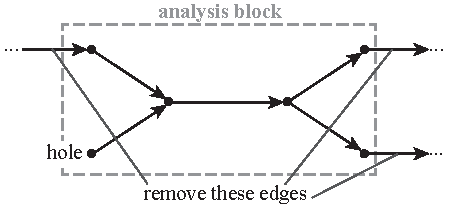
\includegraphics[width=3in]{images/analysis_block_hole}
        \end{center}
        \vspace{-20pt}
    \caption{Example variable node indicating a hole.}
    \label{f:hole}
    \end{figure}

    \item[\bf{Step 2: Collisions}] 
        The second step is to detect collisions and to disconnect precisely the number of connection edges required such that all collisions are resolved without introducting holes. 
        The set of variable nodes at which collisions occur is 
    \begin{equation}
    S_\txt{nodes} = \{v \in V_{M,\txt{var}} \st \txt{deg}^-(v) > \txt{deg}_u^-(v) \},
    \end{equation}
where the degree is now calculated with respect to $F_1$.
    For each collision node we can construct a set containing the edges directed into the node. The set containing all of these sets is constructed as
    \begin{equation}
        S_\txt{edges} = \big \{ \{(x,y) \in E_M\} \ \big| \ y \in S_\txt{nodes} \big \}
    \end{equation}
    Let $J=\{1,2,\ldots,|S_\txt{edges}|\}$ be an indexing set for $S_\txt{edges}$ such that each $S_{\txt{edges},j}$ corresponds to a set in $S_\txt{edges}$ for $j \in J$. 
    An example collision is shown in Fig.~\ref{f:collision} to exemplify the definition of $S_{\txt{edges},j}$. 
    $J$ also indexes $S_\txt{nodes}$ because there is a one--to--one correspondence between the elements in $S_\txt{nodes}$ and the elements in $S_\txt{edges}$ (which are sets). 
    We may then construct sets of edges as
\begin{IEEEeqnarray*}{rCl}
    B_j =  &\big\{& e_k \in S_{\txt{edges},j} \st k \in \{1,2,\ldots,K\} \\
& & \txt{ with } \txt{deg}_u^-(v_j) \leq K \leq \txt{deg}_u^-(v_j) \big \}, \ j \in J,
\end{IEEEeqnarray*}

        which means that each set $B_j$ is constructed from the set $S_{\txt{edges},j}$ by taking only as many edges as are allowed by the upper and lower indegree limits of $v_j$.  
The construction of each $B_j$ corresponds to making a decision about which edges to include and which edges not to include. 
Let the new set of connection edges be denoted
    \begin{equation}
    E_{F_2,\txt{con}} = \{ e \in E_{F_1,\txt{con}} \st e \in B_j \txt{ for some } j \in J\}.
    \end{equation}
The set of all edges is created by removing the connection edges not in $E_{F_2,\txt{con}}$:
    \begin{equation}
    E_{F,2} = E_{F_0} \setminus (E_{M,\txt{con}} \setminus E_{F_2,\txt{con}}),
    \end{equation}
    which gives
    \begin{equation}
    F_2 = (V_{F_0},E_{F_2}).
    \end{equation}
    \begin{figure}[htb!]
        \begin{center}
        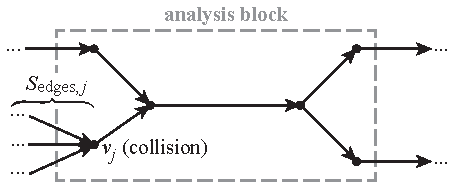
\includegraphics[width=3in]{images/analysis_block_collision}
        \end{center}
        \vspace{-20pt}
    \caption{Example variable node indicating a collision.}
    \label{f:collision}
    \end{figure}

    \item[\bf{Step 3: Finalize}] 
        The third and final step is to prune the graph to exclude any analysis blocks that became unneeded after the collisions were resolved.
        This is accomplished by first creating the reverse graph of $F_2$, $R = (V_R,E_R)$, where
	\begin{equation}
	E_R = \{ (x,y) \st (y,x) \in E_{F_2}\}, \ V_R = V_{F_2}
	\end{equation}
	Next, a new node $b$ is added to $V_R$ and edges directed from this node to each of the expression blocks are added:
    \begin{equation}
        \forall i \in I_E,\forall v \in V_{E_i}, \txt{ if } \txt{deg}^-(v)=0 \txt{ then } (b,v) \in E_R.
    \end{equation}
        The set of nodes that may be reached from $b$ is then constructed as
    \begin{equation}
        U = \{ v \in V_R \st \exists P \txt{ a path from $b$ to $v$}, \ P \subset R \}.
        \end{equation}
	Because $b$ is directed into only the expression blocks, any path from $b$ necessarily provides a path from at least one expression block, which means the node is being used in the problem formulation.

        The list of analysis blocks with at least one node in $U$ is constructed as
        \begin{equation}
        I_F = \{ i \in I_A \st V_{A_i} \cap U \neq \emptyset \}
        \end{equation}
        Any analysis block not in $I_F$ should be removed from the graph because none of its outputs contribute to the problem. Inputs that are not being used are also removed. The set of nodes to remove is then
        \begin{equation}
        N = (V_\txt{in}\setminus U )  \cup \left( \bigcup_{i \notin I_F} V_{A_i} \right),
        \end{equation}
and the new set of nodes is created as
        \begin{equation}
        V_F = V_{F_2} \setminus N.
        \end{equation}
        Edges involving the removed nodes are also deleted as
        \begin{equation}
        E_F = E_{F_2} \setminus \{ (x,y) \st x \in N \txt{ or } y \in N  \}.
        \end{equation}

The fundamental problem graph is then
\begin{equation}
F = (V_F,E_F).
\end{equation}
        If desired, the set of connection edges can be extracted by considering only edges whose endpoints are not in the same analysis block:
\begin{IEEEeqnarray*}{rCl}
E_{F,\txt{con}} = &\{&(x,y) \in E_{F} \st \sim(x \in V_{A_i} \txt{ and } y \in V_{A_i}  \\
& & \txt{for some } i \in I_F)\}.
\end{IEEEeqnarray*}
\end{description}

This algorithm will always provide an FPG if one exists. If an FPG does not exist, the implementation reveals the limiting factors that prevent a valid FPG from being achieved.

\subsection{Suggested Process for Appyling the FPG Algorithm}
\label{ss:process}
Section \ref{ss:obtaining FPG} provided an algorithm for obtaining an FPG from the given MCG. 
The algorithm can be applied as part of a broader process in which the designer changes the problem formulation or the supplied analysis tools to attempt to obtain an FPG. The following steps detail the suggested procedure for obtaining an FPG:
\begin{enumerate}
\item[\bf{(A)}] Begin with a set of inputs, analysis tools, objectives, and constraints.
\item[\bf{(B)}] Build the MCG as described in Sec.~\ref{ss:MCG}.
\item[\bf{(C)}] Set indegree limits for variable nodes representing local inputs as described in Sec.~\ref{s:indegree-outdegree} and Table \ref{t:variable node classification}.
\item[\bf{(D)}] Run the FPG algorithm described in Sec.~\ref{ss:obtaining FPG}. If a valid FPG is unattainable:
		\begin{enumerate}
\item Change the MCG by adding analysis blocks and/or inputs, which means identifying new analysis tools to include in a potential MDAO workflow.
\item Change indegree limits (see Table \ref{t:variable node classification}).
\end{enumerate}
\item[\bf{(E)}] Repeat from step (A) until an FPG is obtained.
\end{enumerate}
This process illustrates how the algorithm for obtaining a valid FPG can be applied. However, the process also serves to illustrate how a designer may revist the MCG after an FPG has already been produced. For example, if a designer desires to change an input to be multi-fidelity, new analysis blocks can be added to the original MCG, the indegree limits can be modified accordingly, and the algorithm can be applied again.



\subsection{Problem Solution Graph}
Once a suitable FPG has been obtained the issue of how to structure a solution strategy 
can be addressed. Similar to the way an MCG can be manipulated into a FPG, an FPG can be
further manipulated into a PSG. To get from an MCG to an FPG you eliminated analysis blocks and
connection edges to reduce the problem to something solvable, but to get from an FPG to a PSG you 
add in driver blocks, driven edges to describe the structure of the solution strategy being applied 
to the problem. For example, Figure \ref{f:sellar_psg} shows the PSG that solves the Sellar problem 
with an MDF solution strategy. There are two driver blocks in this PSG, one for the solver that 
ensures compatibility and another for the optimizer that picks the design variables. 

\begin{figure}[htb]
    \begin{center}
    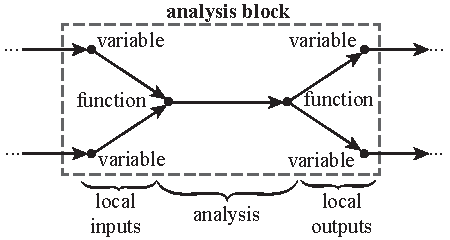
\includegraphics[width=3.0in]{images/sellar_mdf_psg}
    \end{center}
    \vspace{-10pt}
    \caption{Example PSG for solving the Sellar problem with MDF strategy}
    \label{f:sellar_psg}
\end{figure}

The PSG in figure \ref{f:sellar_psg} can be compared to the XDSM for the same situation 
in Fig. \ref{fig:XDSM_simple}. While the two diagrams contain much of the same information 
there is a significant difference. The PSG describes the data passing that happens between 
the drivers and the rest of the problem, but it does not describe when that data passing 
will occur (the execution order of the blocks). In the proposed graph syntax edges describe 
the passing of data between one node an another, but they do not define when that 
communication happens. 

XDSM diagrams do contain information about data passing as well as when that data should be passed. 
XDSM essentially represents two related, but independent graphs simultaneously. 
This is accomplished by including two distinct sets of edges, one for data 
connections and a second indicating execution sequence. As seen in Fig. \ref{fig:XDSM_simple}
data connections are bold-gray edges and execution connections are numbered-black edges. The
execution edges, the back edges, in XDSM represent and additional graph that
follows a completely different set of rules and behaviors from the data connections graph. 
On the other hand the data described by the gray edges, 
the data passing information, is equivalent to the information in the PSG. XDSM presents this 
information in a more compact and human readable manner by aggregating groups of related variables
into combined nodes. The more verbose form presented in a PSG is less human readable, but more easily 
machine readable as a consequence of a more consistent structure. 



